\documentclass{scrreprt}
\usepackage{etex}
\usepackage[ngerman]{babel}
\usepackage[utf8]{inputenc}
\usepackage[T1]{fontenc}
\usepackage{amsmath, amssymb}
\usepackage{graphicx}

\usepackage{pgfplots}
\pgfplotsset{compat=1.11}
\usepgfplotslibrary{external}
\usepackage{pgfplotstable}

\usepackage{booktabs}
\usepackage{multirow}
\usepackage{longtable}
%\usepackage{ulsy}
%\usepackage{pst-all}
\usepackage{picture}
\usepackage[automark]{scrpage2}
\usepackage{caption}
\pagestyle{scrheadings}
\ihead[]{Friedrich Hübner 2897111}
\ohead[]{Fiona Paulus 2909625} 

\author{Friedrich Hübner 2897111\\
Fiona Paulus 2909625}
\title{Computerphysik\\Hausarbeit 5}

\begin{document}
\maketitle
\newpage

\chapter*{Der Differentialgleichungssolver für Runge-Kutta-Verfahren}
Für den DGL-Solver wurde das Runge-Kutta-Verfahren mit den Fehlbergkoeffizienten und das klassische Runge-Kutta-Verfahren programmiert. Die Berechnung aller Werte erfolgt genau nach diesen Verfahren. Der Solver wird sowohl in Aufgabe 1 als auch 2 mit den entsprechenden Koeffizienten benutzt. 

\section*{Programm (abgabe4\_runge\_kutta.cpp)}
In dieser Datei befindet sich das Runge-Kutta-Verfahren analog zur Hausarbeit 4.\\

In der Datei wird die Klasse RungeKutta definiert, die einen DGL-Solver darstellt. diese hat folgende Funktionen:
\begin{itemize}
	\item Konstruktor: RungeKutta(f,$t_0$,$y_0$, algo): Er initialisiert einen DGL-Solver mit der Funktion f ($y' = f(t,y)$), die Anfangszeit $t_0$, den Anfangsvektor $y_0$ und einem Koeffizientenset algo. Dabei ist algo vom Typ struct RungeKuttaAlgorithm, was im wesentlichen eine Sammlung aller Koeffizienten eines Verfahrens ist. Dies ermöglicht eine einfache Auswahl aus vorher schon definierten Koeffizientensets. In der Datei befinden sich die beiden RungeKuttaAlgorithm-Instanzen fehlberg und classic, die jeweils das entsprechende Verfahren darstellen. 
	\item iterate(): berechnet einen neuen Schritt und gegebenenfalls die neue optimale Schrittweite
	\item setStepSize(h): setzt die aktuelle Schrittweite auf h
	\item set Precision(p): setzt das $\varepsilon$ für die Schrittweitensteuerung auf p
\end{itemize}

Außerdem werden in der Datei Operatoren für Vektorarithmetik (+,+=,-,*) und für Ausgabe von Vektoren (<\.<) überladen. Zusätzlich gibt es noch Funktionen für den Betrag von Vektoren und das Skalar- und Kreuzprodukt.  


\chapter*{Aufgabe 3}
\section*{Allgmeine Hinweise}
Das Programm wurde unter Windows 10 mit "g++ -o abgabe55\_3.exe -Wall -Wextra -std=c++0x -O2 -static abgabe5\_3.cpp"\;kompiliert.

\section*{a) (aufgabe3.cpp)}
In der Datei befindet sich die Funktion numerov, die die Schrödingergleichung bei einer Energie e mit 2 Anfangswerten und dem Potential 'potential' löst. Die Funktion gibt ein Array der y-Werte zurück, wobei $y_i = y(h \cdot i)$, h Schrittweite.

\subsection*{Symmetriebetrachtungen}
Da die Potentiale in beiden Fällen symmetrisch sind, gibt es nur symmetrische und antisymmetrische Wellenfunktionen. Nummeriert man die Zustände aufsteigend nach ihren Energien durch (beginnend bei 0 für den Grundzustand), so haben alle geraden Zustände symmetrische und alle ungerade Zustände antisymmetrische Wellenfunktionen. Das es nur gerade und ungerade Lösungen gibt, reicht es nur eine Hälfte der Funktion zu berechnen, nämlich $x\in [0,\infty]$.\\

\subsection*{Anfangswerte}
Da die Schrödingergleichung linear ist, reicht es, eine beliebige unnormierte Lösungsfunktion zu einer bestimmten Energie zu finden und später zu normieren.
Mit diesen Überlegungen kommt man zu folgenden Anfangsbedingungen:
\begin{itemize}
	\item symmetrische Lösungen: $y(0) = 1, y'(0)=0$, bzw. $y_0 = y_1 = 1$. Jede symmetrische Lösung hat Ableitung 0 bei 0. Der Wert $y(0) = 1$ ist vollkommen willkürlich, kann aber später durch normieren nachträglich angepasst werden (siehe b)).
	\item antisymmetrische Lösungen: $y(0) = 0, y'(0) = 1$, bzw. $y_0 = 0, y_1 = h$, mit h der Schrittweite. Jede antisymmetrische Lösung muss $y(0) = 0$ haben. Der Anstieg $y'(0) = 1$ ist wieder vollkommen willkürlich und wird durch die Normierung nachträglich geändert. 
\end{itemize}

\section*{b)}
Anmerkung: Alle Energien werden in vielfachen von $\hslash \omega$ angegeben.\\

Für den harmonischen Oszillator wird als Potential die Funktion 'harmonicOscillator' benutzt. Es wird von 0 bis 10 integriert. Dabei ergibt sich typischerweise folgendes Bild:
\begin{center}
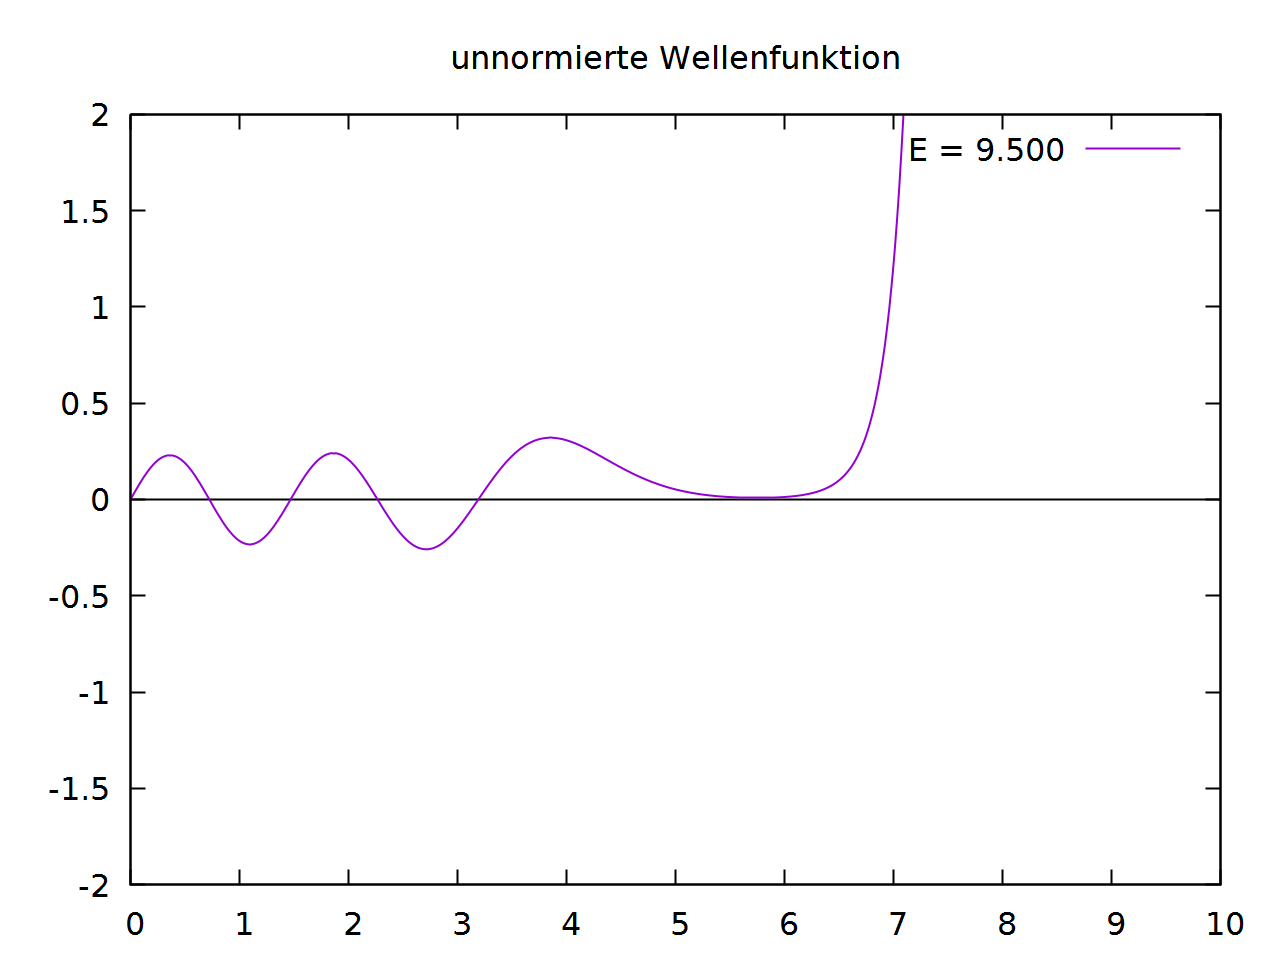
\includegraphics[scale=0.3]{aufgabe3/plot_unnorm.png}
\captionof{figure}{Unnormierte Wellenfunktion}
\end{center}

Man kann erkennen, dass die Funktion gut integriert wird, dann gegen 0 abfällt und dann plötzlich nach $\infty$ abknickt.

\subsection*{Normierung}
Um die Norm der Wellenfunktion zu bestimmen, berechnet man das Integral über das Betragsquadrat der Wellenfunktion. Dies geschieht mit der zusammengesetzten Trapezmethode. Da wir die Funktion nur für positive x kennen, wird das Integral nur für positive x berechnet und danach verdoppelt. Das Integral wird bis zum Abknickpunkt berechnet, da danach die Wellenfunktion nicht mehr realistisch ist. Das Integral geht also von 0 bis zum Abknickpunkt.

\subsubsection*{Bestimmung des Abknickpunkts}
Um den Abknickpunkt zu bestimmen, kann man sich zu nutze machen, dass die n. Eigenfunktion genau Nullstellen hat, bzw. im Intervall $(0,\infty)$ genau $\lfloor n/2\rfloor$. Danach steigt die Funktion (genauer: deren Betragsquadrat) noch einmal kurz an und fällt dann wie $\exp{-x^2}$ ab. Beim Abknickpunkt gibt es dann ein lokales Minimum der Funktion.\\

Der Algorithmus geht jetzt wie folgt vor: Er geht alle berechneten Funktionswerte Schrittweise durch. Der Algorithmus zählt jetzt die Anzahl der Nullstellen (Nulldurchgänge) der Wellenfunktion. Hat er $\lfloor n/2\rfloor$ Nullstellen gefunden, so sucht er nach dem nächsten lokalen Minimum des Betragsquadrates der Wellenfunktion. An diesem Punkt wird dann die Integration abgebrochen.\\

Die gesamte Prozedur zur Bestimmung der Norm wird durch die Funktion getNorm(psi, zeros) beschrieben. Dabei ist psi die Wellenfunktion als Array gegeben und zeros die Anzahl der zu erwartenden Nullstellen. Der Rückgabewert ist ein Paar (double, int) mit der Norm und dem Index des Abknickpunktes. In den späteren Graphiken wurde die Wellenfunktion an dem Abknickpunkt abgeschnitten, um eine größere Übersicht zu gewährleisten.

\subsection*{Bestimmung der Grundzustandswellenfunktion}
Aus der theoretischen Physik ist bekannt, das die Grundenergie bei 0.5 liegen sollte. In der Umgebung von 0.5 sehen die Wellenfunktionen folgendermaßen aus:

\begin{center}
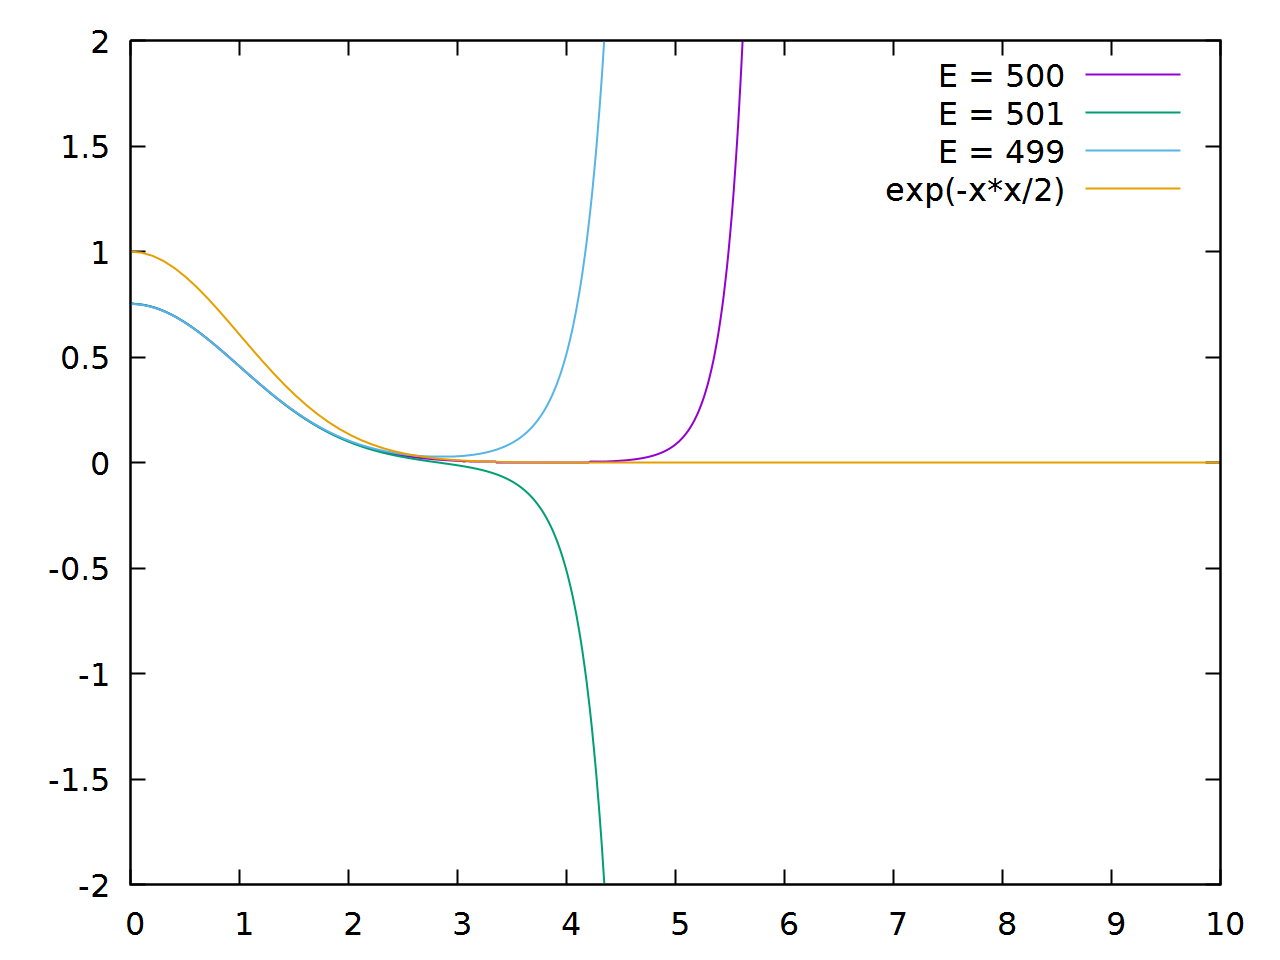
\includegraphics[scale=0.3]{aufgabe3/plot_ground.png}
\captionof{figure}{Bestimmung des Grundzustandes}
\end{center}

Ein Energieeigenwert zeichnet sich dadurch aus, dass die Wellenfunktion im unendlichen gegen 0 geht. In dem Bild kann man erkennen, dass die Funktion für $E=0.5$ gegen unendlich geht und für $E = 0.501$ gegen minus unendlich. Somit muss zwischen beiden Energien eine Lösung der Schrödingergleichung liegen. Also ist die Grundzustandsenergie: $E = 0.5 \pm 0.001$.\\

Im nächsten Bild ist die Abweichung der Funktion für $E = 0.5$ von der theoretischen Lösung $1/\pi^{(1/4)}\exp{-x^2/2}$ bis zum Abknickpunkt ($x\approx 3$) dargestellt:

\begin{center}
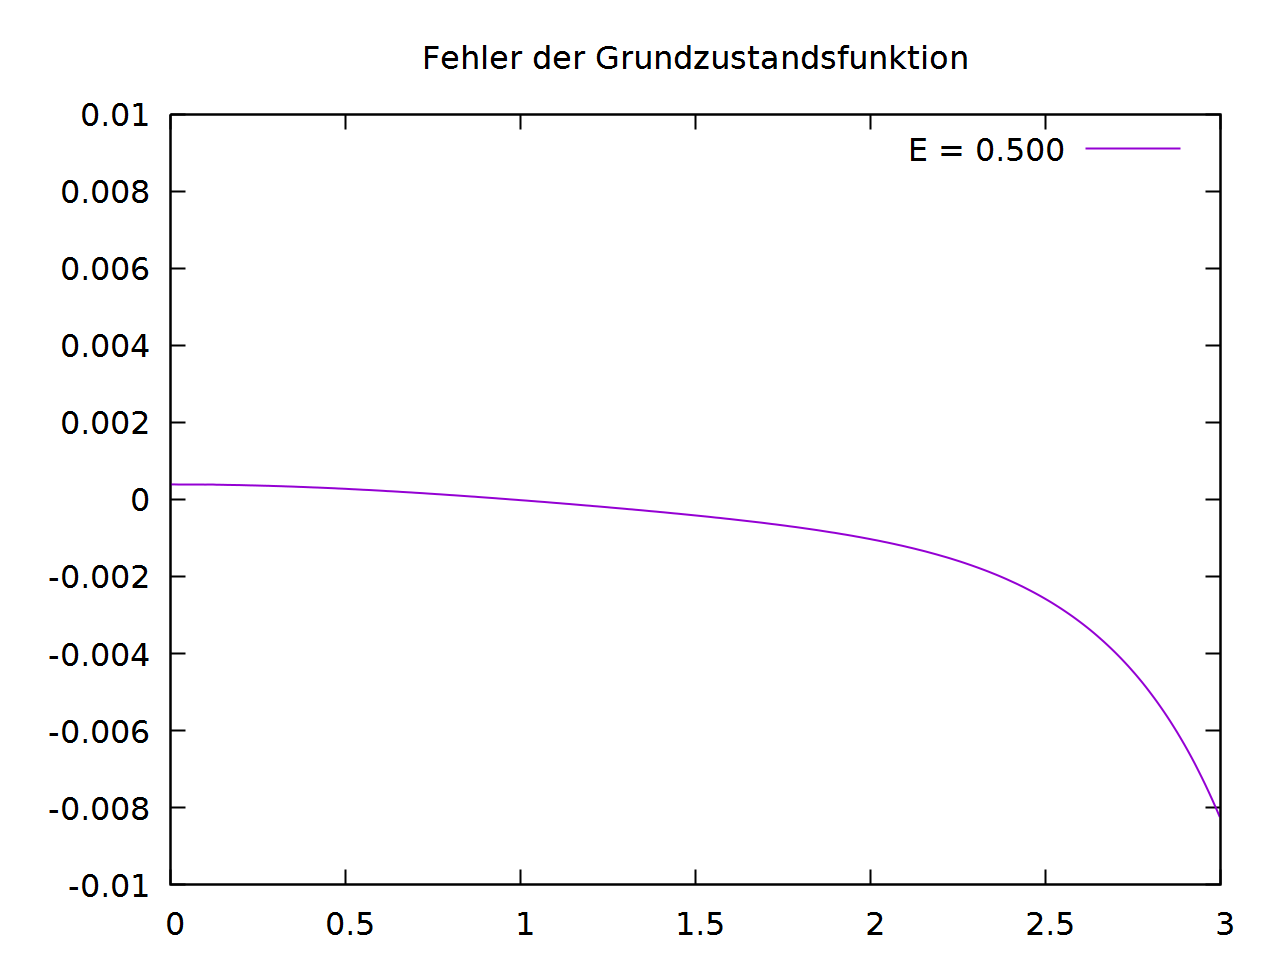
\includegraphics[scale=0.3]{aufgabe3/plot_ground_diff.png}
\captionof{figure}{Fehler des Grundzustandes}
\end{center}

Der Fehler ist im Vergleich zu der Funktion recht klein, er wird aber für große x zunehmend größer. Da die Funktion für große x gegen 0 geht, ergibt sich hier ein recht großer relativer Fehler ($\approx 100\%$). Ansonsten scheint das Ergebnis recht gut zu sein.

\section*{c)}
Man kann erwarten, dass die Energieeigenwerte etwa einen Abstand von $\hslash \omega = 1$ haben. Um die Energien zu bestimmen, geht man immer Energiewerte in kleineren Abständen (hier 0.1) durch und berechnet die zugehörige Wellenfunktion.\\
Analog zur Bestimmung des Grundzustandes, ist ein Energieeigenwert dadurch gegeben, dass die Funktion im unendlichen gegen 0 geht. Für alle anderen Energien divergieren die Funktionen. Stellt man jetzt bei der Erhöhung der Energie um $E_{i+1} = E_i + 0.1$ fest, dass sich das Divergenzverhalten von $-\infty$ zu $\infty$ oder andersherum ändert, so liegt im Intervall $[E_i, E_{i+1}]$  ein Energieeigenwert.\\
Auf diesem Intervall wird dann ein Bisektionsverfahren durchgeführt. Als Vergleichskriterium wird immer der Wert der Wellenfunktion bei 10 genommen. Dessen Vorzeichen bestimmt, ob die Funktion gegen + oder - $\infty$ geht. Das Bisektionsintervall wird immer so angepasst, dass der linke Rand und der rechte Rand ein unterschiedliches Divergenzverhalten haben. Die Bisektion wird abgebrochen, wenn das Intervall kleiner als 0.001 geworden ist. Somit hat man einen Energieeigenwert auf 0.001 genau bestimmt.\\

Dieses Verfahren wird durch die Funktion 'sweep()' realisiert. Es gibt ein Array von Paaren (double, bool) zurück. Der erste Wert ist der Energiewert, der zweite Wert ist wahr, wenn es sich um eine symmetrische Funktion handelt, sonst falsch.

\section*{d)}
Jetzt wird das Potential 'anharmonicOscillator' verwendet. Die Energieeigenwerte sind: $0.885, 3.043, 5.800, 8.929, 12.357, 16.038, 19.939, 24.036, 28.315, 32.758$:

\begin{center}
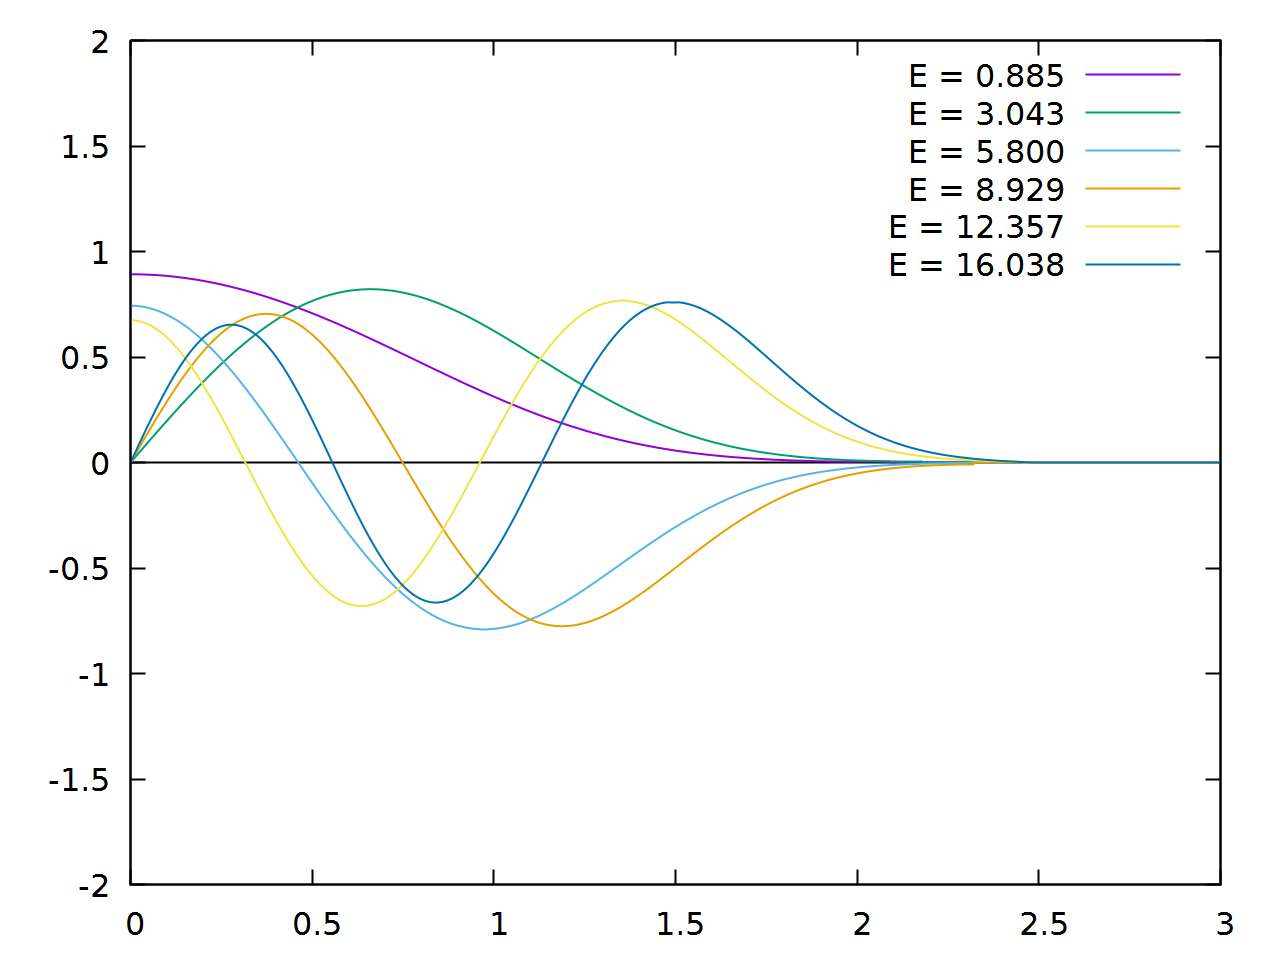
\includegraphics[scale=0.3]{aufgabe3/plot_sweep_perturbation_cut.png}
\captionof{figure}{Die ersten 5 symmetrischen und antisymmetrischen Lösungsfunktionen}
\end{center}

\section*{Sonstige abgegebene Dateien}
\subsection*{plot\_harmonic.plt, plot\_sweep\_perturbation.plt}
Die Plot-Dateien für das normale und das gestörte Potential
\subsection*{out\_[E].txt}
Die Ausgabedateien des Programmes. Entspricht immer einer Wellenfunktion mit der Energie E/1000.
\subsection*{out\_sweep\_perturbation\_[E].txt}
Das gleiche wie oben, nur für den gestörten Oszillator
\end{document}